\frame{
    \frametitle{Initialization of the SOM}
    The SOM is initialized randomly with an uniform distribution within the range of the input data.
    \begin{columns}
        \begin{column}{.6\textwidth}
            \begin{center}
                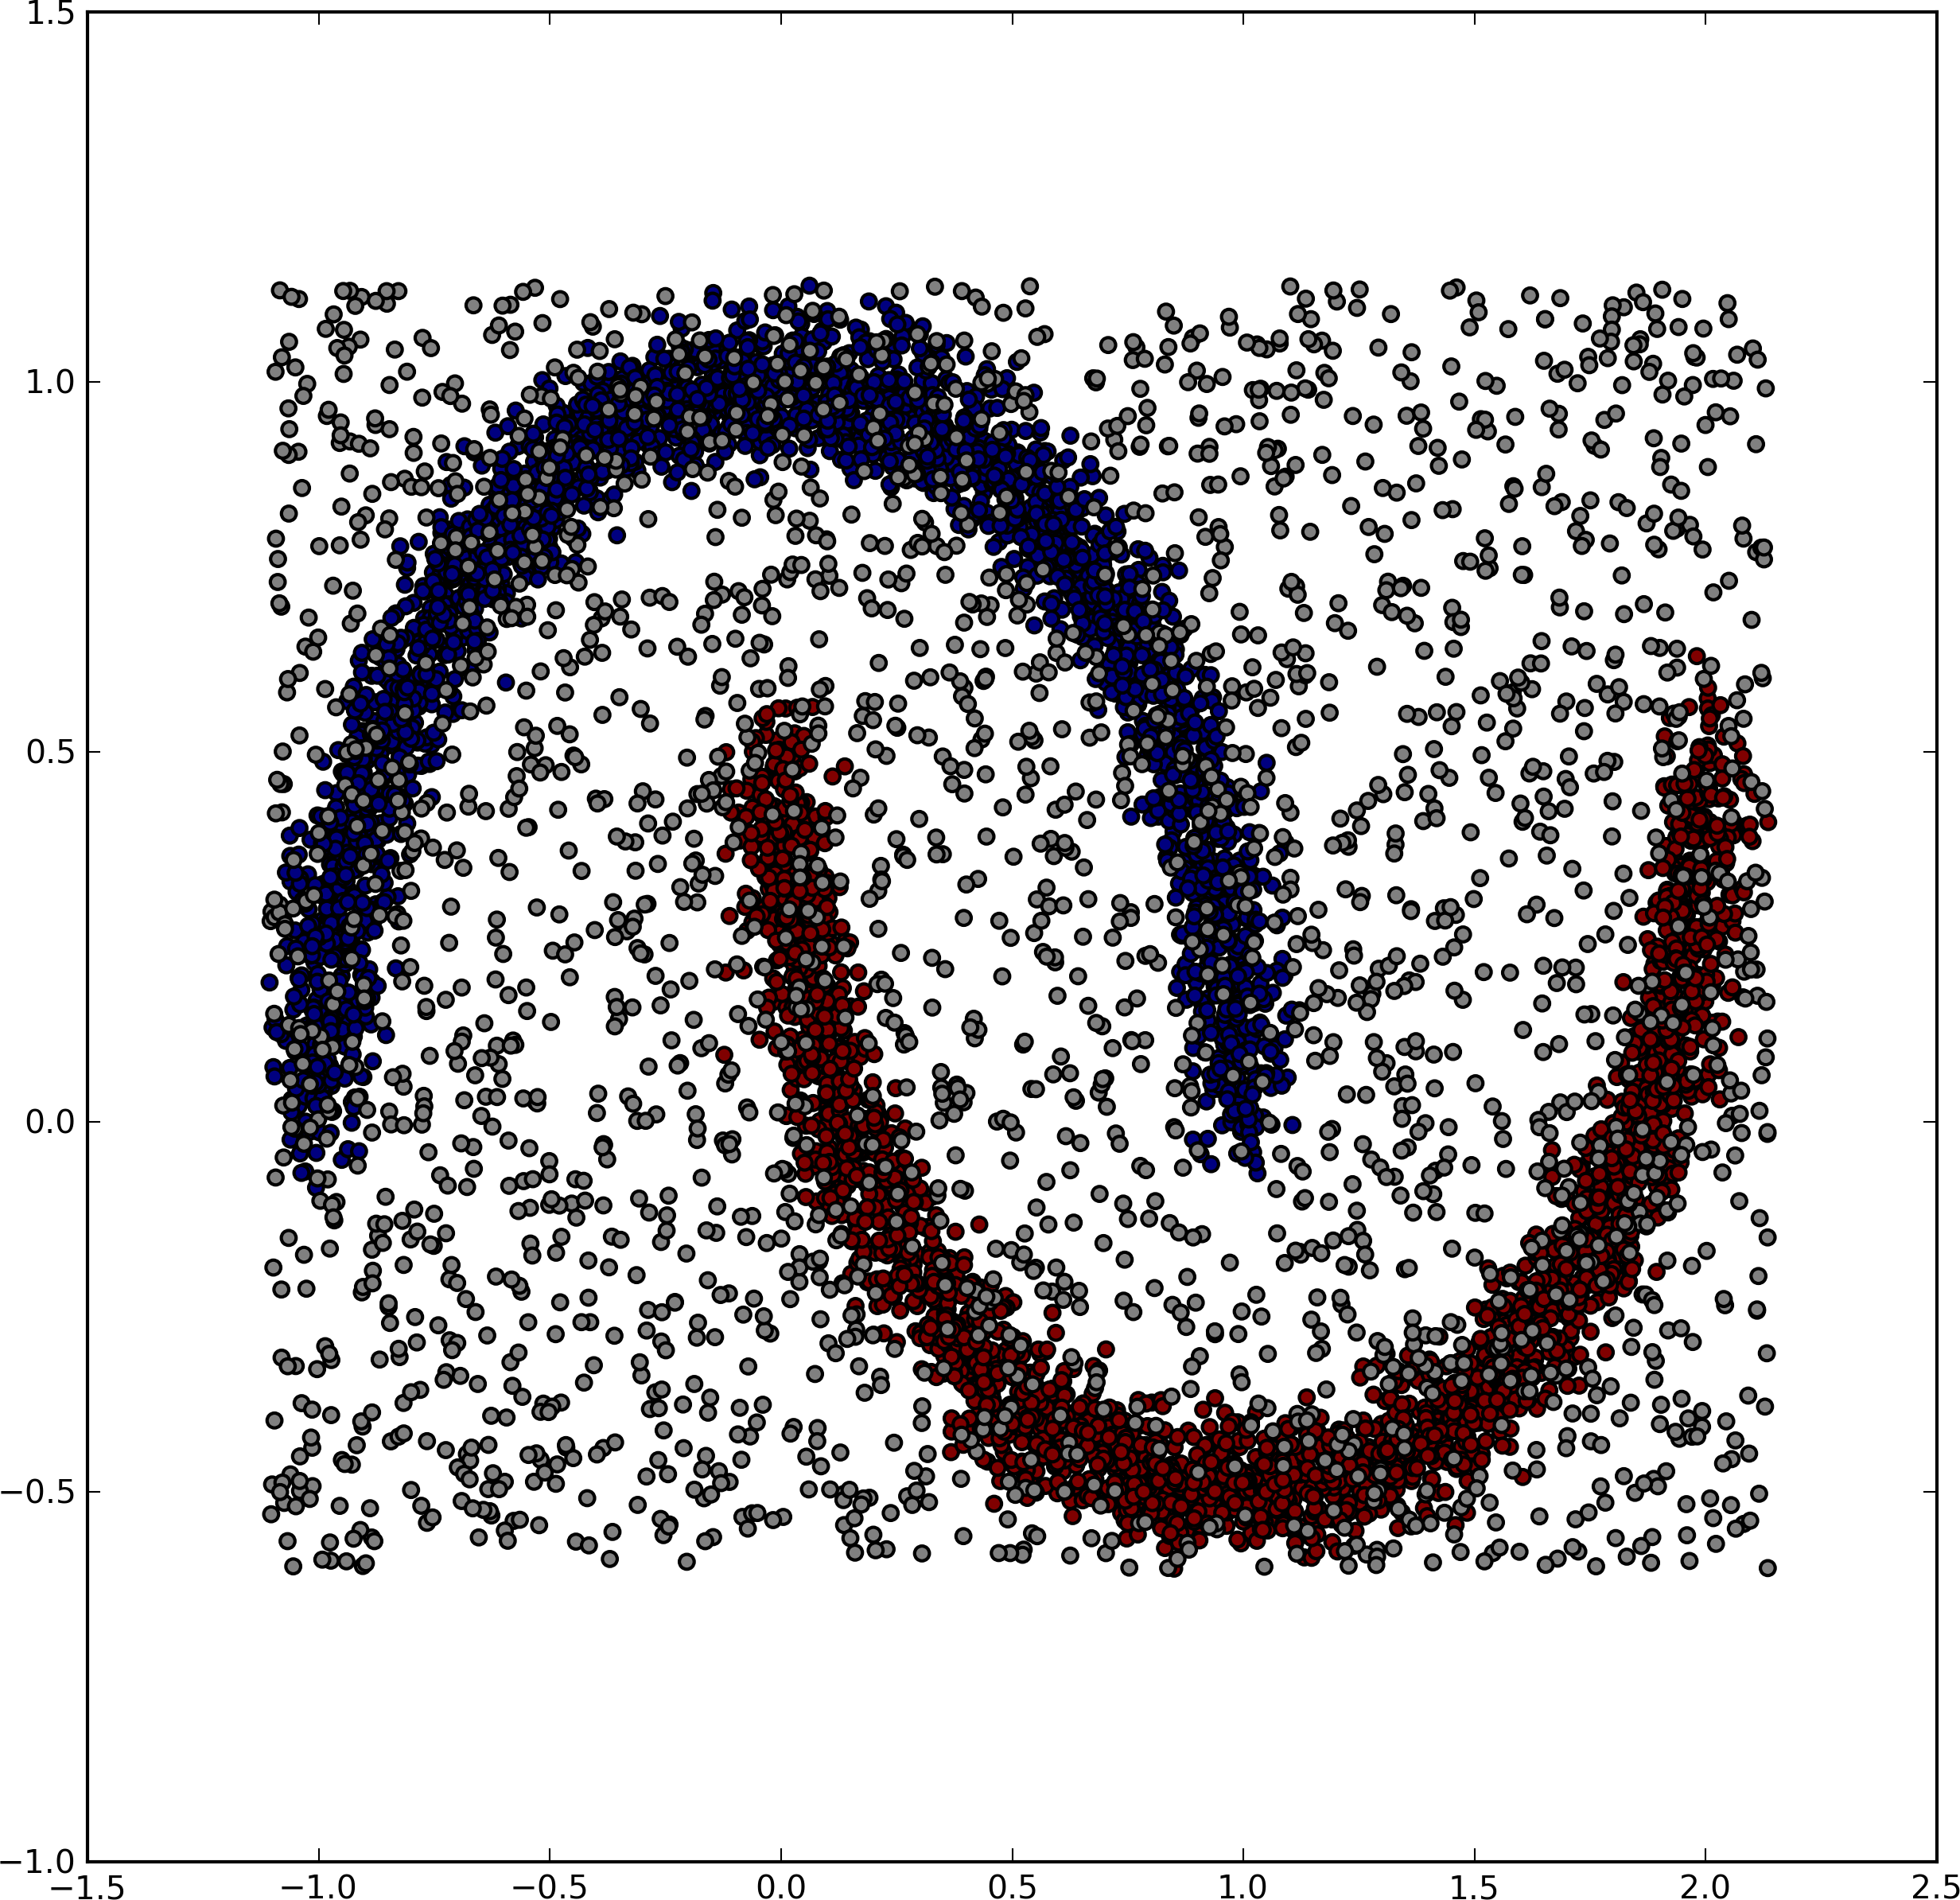
\includegraphics[width=\textwidth]{figures/sominit.png}
            \end{center}
        \end{column}
        \begin{column}{.4\textwidth}
            Example of SOM initialization on the moon dataset. 
            Take care to differentiate the \textbf{SOM space} which is a \textbf{2D lattice} of 2D vectors for this example and the \textbf{input space}, represented on the left.
        \end{column}
    \end{columns}
}
